\section{The numbers of \protein{BubR1}, \protein{Bub1}, and \protein{Mad1} recruited per signaling kinetochore are inversely correlated with the total number of signaling kinetochores in the cell}

We decided to quantify the copy number of SAC proteins recruited by individual signaling kinetochores to assess their steady state signaling activity. We focused on one protein each from the three layers of the recruitment cascade: Bub1, BubR1, and Mad1.

To ensure accurate quantification and comparative analysis, we used genome-edited HeLa cells that express either mNG-Bub1, mNG-BubR1, or Mad1-mNG. Because the fluorescent tags are separated from the tagged proteins by flexible linkers, we assume that signaling kinetochores recruit roughly equal amounts of tagged and untagged proteins.

Our goal was to characterize the dependence of Bub1, BubR1, and Mad1 recruitment per kinetochore on the total number of signaling kinetochores in the cell. We obtain mitotic cells containing distinctly different numbers of signaling kinetochores using two drugs.

To obtain cells with nearly all kinetochores unattached, we released G1/S arrested HeLa cells into the cell cycle and then arrested them in mitosis using nocodazole, a drug that depolymerizes microtubules. These cells serve as a model for cells right after the NEBD.

To obtain mitotic cells with a much smaller number of signaling kinetochores, we released G1/S arrested HeLa cells into the cell cycle and treated them with GSK923295, a small molecule inhibitor of the mitotic kinesin CENP-E \cite{GSK923295}. In these cells, a variable, but smaller, number of chromosomes stranded near the spindle poles (Figure 1B, left). Kinetochores on these chromosomes are either unattached or laterally attached, and they activate the SAC by recruiting SAC signaling proteins \cite{GSK923295LateralAttachmentEM, GSK923295MonastrolCotreatment}. The remaining chromosomes align at metaphase plates, and their kinetochores recruit significantly lower amounts of SAC proteins. These cells serve as the model for cells near the end of the prometaphase. Because the number of signaling kinetochores is variable in GSK923295-treated cells, we analyzed only those cells that contained 10 or less than 10 polar chromosomes based on a visual inspection of the $z$-stack.

BubR1 and Mad1 recruitment per kinetochore in nocodazole-treated cells was lower than the Bub1 recruitment. In GSK923295-treated cells, the recruitment per kinetochore was significantly higher for all three proteins. Taken together with the data from nocodazole-treated cells, these measurements suggest that the number of SAC proteins recruited per kinetochore is inversely correlated with the number of signaling kinetochores in the cell. This trend is consistent with observations made in budding yeast (Aravamudhan et al., 2016).

It should be noted that Mad1-Mad2 is recruited to metazoan kinetochores as well as the fibrous coronae (Pereira et al., 2018; Rodriguez-Rodriguez et al., 2018; Silio et al., 2015). To quantify the fraction of Mad1-Mad2 recruited by RZZ, we knocked down the Zw10 subunit of the RZZ complex using RNA interference (RNAi) in the three cell lines and then quantified the recruitment of the mNG-labeled SAC proteins to signaling kinetochores as before. ZW10 siRNA treatment resulted in a ~ 25\% decrease in Bub1 and BubR1 recruitment, as noted by others (Kops et al., 2005). As expected, Mad1 recruitment was significantly lower in both GSK923295 and nocodazole-treated cells (\myref{siZW10SACProteinKinetochoreRecruitment_Quantification}). The number of Mad1 molecules recruited was reduced approximately by half, revealing the contribution of the RZZ under these conditions. The number of Bub1 and BubR1 molecules per kinetochore was also reduced. However, the number of SAC proteins recruited per kinetochore is still inversely correlated with the number of signaling kinetochores in the cell.

We then asked whether the differences between nocodazole- and GSK923295-treated groups were correlated with differential recruitment of these SAC proteins at signaling kinetochores and if so, whether these differences were contributed by \protein{Knl1} or the fibrous coronae (which is disrupted by \gene{ZW10} knockdown). Using wide-field fluorescence Microscopy, we determined that \protein{BubR1}, \protein{Bub1}, and \protein{Mad1} recruitment at signaling kinetochores are all enhanced when cells were treated with GSK923295 compared with nocodazole (\myref{SACProteinKinetochoreRecruitment_Quantification}).

\begin{figure}
    \centering
    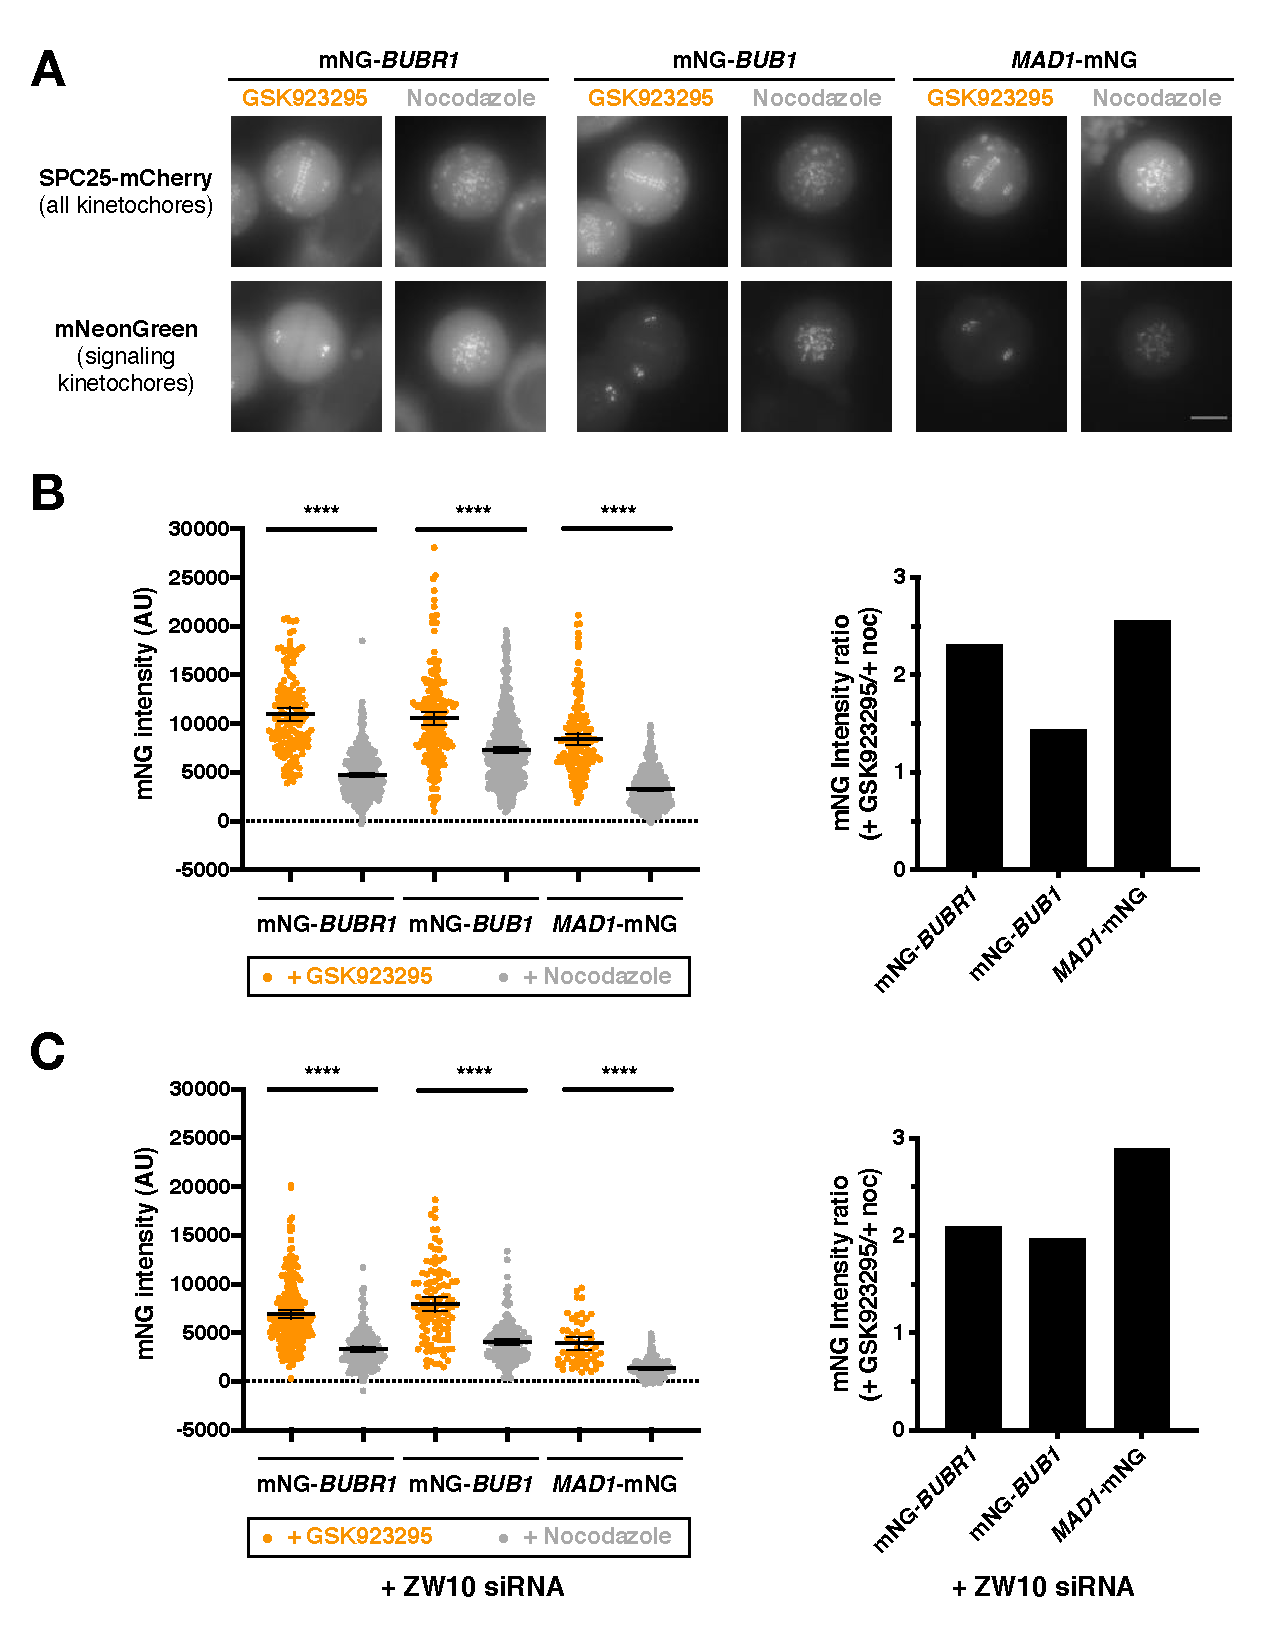
\includegraphics[width=\textwidth]{chapters/figures/SACProteinKinetochoreRecruitment.pdf}
    \phantomsubfiglabel{SACProteinKinetochoreRecruitment_Images} % subfigure A
    \phantomsubfiglabel{SACProteinKinetochoreRecruitment_Quantification} % subfigure B
    \phantomsubfiglabel{siZW10SACProteinKinetochoreRecruitment_Quantification} % subfigure C
    \caption{\textbf{\protein{BubR1} is more influential to SAC signaling strength and enriched at the few signaling kinetochores in GSK923295-treated cells than \gene{Bub1} and \protein{Mad1}.}}
    \noindent\justifying Lauren Humphrey-Stark performed all imaging experiments and data analysis involved in this figure. \myref{SACProteinKinetochoreRecruitment_Quantification,siZW10SACProteinKinetochoreRecruitment_Quantification} were reproduced from one of my first-author manuscripts in preparation. (A) Mitotic duration (NEBD to anaphase onset) of HeLa-A12 cells with \Latin{in situ} mNeonGreen-tagged \gene{BubR1}, \gene{Bub1}, or \gene{Mad1} in the presence of 330 nM nocodazole or 236 nM GSK923295. Cells were transfected with either an mNeonGreen-targeting siRNA to knock down the corresponding SAC gene (left panel) or a negative control siRNA (right panel). (B) Exemplary micrographs showing cells from the three HeLa-A12 cell lines treated with nocodazole or GSK923295. Spc25-mCherry labeled all kinetochores. Scale bar, \SI{10}{\micro m}. (B) Quantification of mNeonGreen signals at individual signaling kinetochores from experiments illustrated in (B). Each dot represents the measurement from one signaling kinetochore. Error bars represent 95\% confidence intervals of the mean. Results from at least two independent experiments are shown. Pairwise ratios between the average mNeonGreen signals at individual signaling kinetochores of GSK923295-treated cells and nocodazole-treated cells in (C).
    % Bub1/BubR1 recruitment data with knockdown of the RZZ complex compared with those with no siRNA deviate greatly from Zhang et al., 2019
\label{SACProteinKinetochoreRecruitment}
\end{figure}


